\chapter{Discussion}
\newpage

This thesis has focused on describing protein conformation as a dynamic property under physiological conditions. Such a description is challenging, and diverse strategies can be employed to study it from different perspectives. Nuclear Magnetic Resonance spectroscopy (NMR) experiments can be employed to measure biophysical properties such as order ($S^{2}$) and flexibility (Random Coil Index), describing backbone and side chain dynamics. Another NMR approach to describe a protein's dynamic conformation is the elucidation of structural ensembles at physiological temperatures. Computationally, Molecular Dynamics (MD) simulations also produce protein structural ensembles, with the particularity that they are presented in a time-series. Both approaches, the coordinate-free measurement of biophysical properties and the elucidation of structural ensembles, have been considered in this thesis. 

\section{Conformational State Propensities and Variability}
\sectionmark{Conf. State Propensities and Variability}

A recurrent theme throughout this work is that protein conformation is better described as an ensemble of structures representing the possible conformations that a protein can adopt and transition among in physiological conditions. Beyond the visualisation of all structures and alignment-derived metrics (\textit{e.g.} RMSD), extracting meaningful information from these ensembles can be challenging. Though these atomic precision structures are key to describing protein conformation, their sole usage to describe a protein's conformational landscape is unlikely to cover all possible conformations. Considering, as an example, a protein with 5 loci, each with 5 possible defined conformations (and assuming they are distant enough not to influence each other), the calculation of all possible protein conformation is subject to combinatorial explosion of $5^{5}=3125$ possible conformations. This highlights the need for new metrics for describing conformational diversity.

In this context, Constava (chapter \ref{chapter:constava}) \cite{gavalda-garcia_data-driven_2024} offers a method capable of leveraging information from these ensembles to produce novel residue-level descriptions of protein conformation. This description can also be applied to interpret structural ensembles in changing or differential conditions, providing additional metrics to perform such a challenging analysis.

\subsection{Probabilistic Definition of Conformational States and its Relation to Free Energy Landscapes}

Six conformational states are probabilistically defined within the backbone dihedral space, representing different dynamic states of traditional secondary structures. Although more conformational states could describe additional unique local conformations, we limited our definition to these six states to ensure that each state was represented by a sufficient number of data points. The data used to fit each of the six Probability Density Functions (PDFs) were selected based on criteria from NMR structural ensembles and interpreted chemical shifts (\figref{overal_figure}) \cite{orlando_shiftcrypt_2020}. 

The NMR-derived definition of these conformational states should therefore make them more suitable to describe protein local conformation in physiological temperatures than crystallography-benchmarked secondary structures. \textcolor{red}{Defining these conformational states using solution NMR data implicitly incorporates the effects of water on protein structure, enabling the analysis of more dynamic conformational states than those typically observed in crystallography}. Specifically, the introduction of the ``Surrounding Helix'' and ``Surrounding Sheet'' conformational states incorporates the concepts of relaxed local conformations, which behave somewhat like an $\alpha$-helix or $\beta$-sheet/strand, but show higher dynamism than their ``Core'' forms. The latter, ``Core'' conformational states, indicate closer resemblance to traditional definitions of $\alpha$-helix or $\beta$-sheet/strand, even at physiological temperatures. 

This distinction accommodates for hybrid behaviours between order and disorder found at physiological temperatures. In contrast, the cryogenic temperatures required for X-ray crystallography and Cryogenic Electron Microscopy (Cryo-EM) facilitate the acquisition of local conformation by reducing the Gibbs free energy in the system. This stabilises proteins into their native conformation, at energy levels that prevent transition to other conformations which are available at physiological temperatures. The separation between ``Core'' and ``Surrounding'' conformational states represent residues that most likely would be assigned to the same secondary structure at cryogenic temperatures (\figref{fig:discussion:surrhelix_vs_xray}), now distinguished in two states. 

\begin{figure}[htb!]
    \centering
    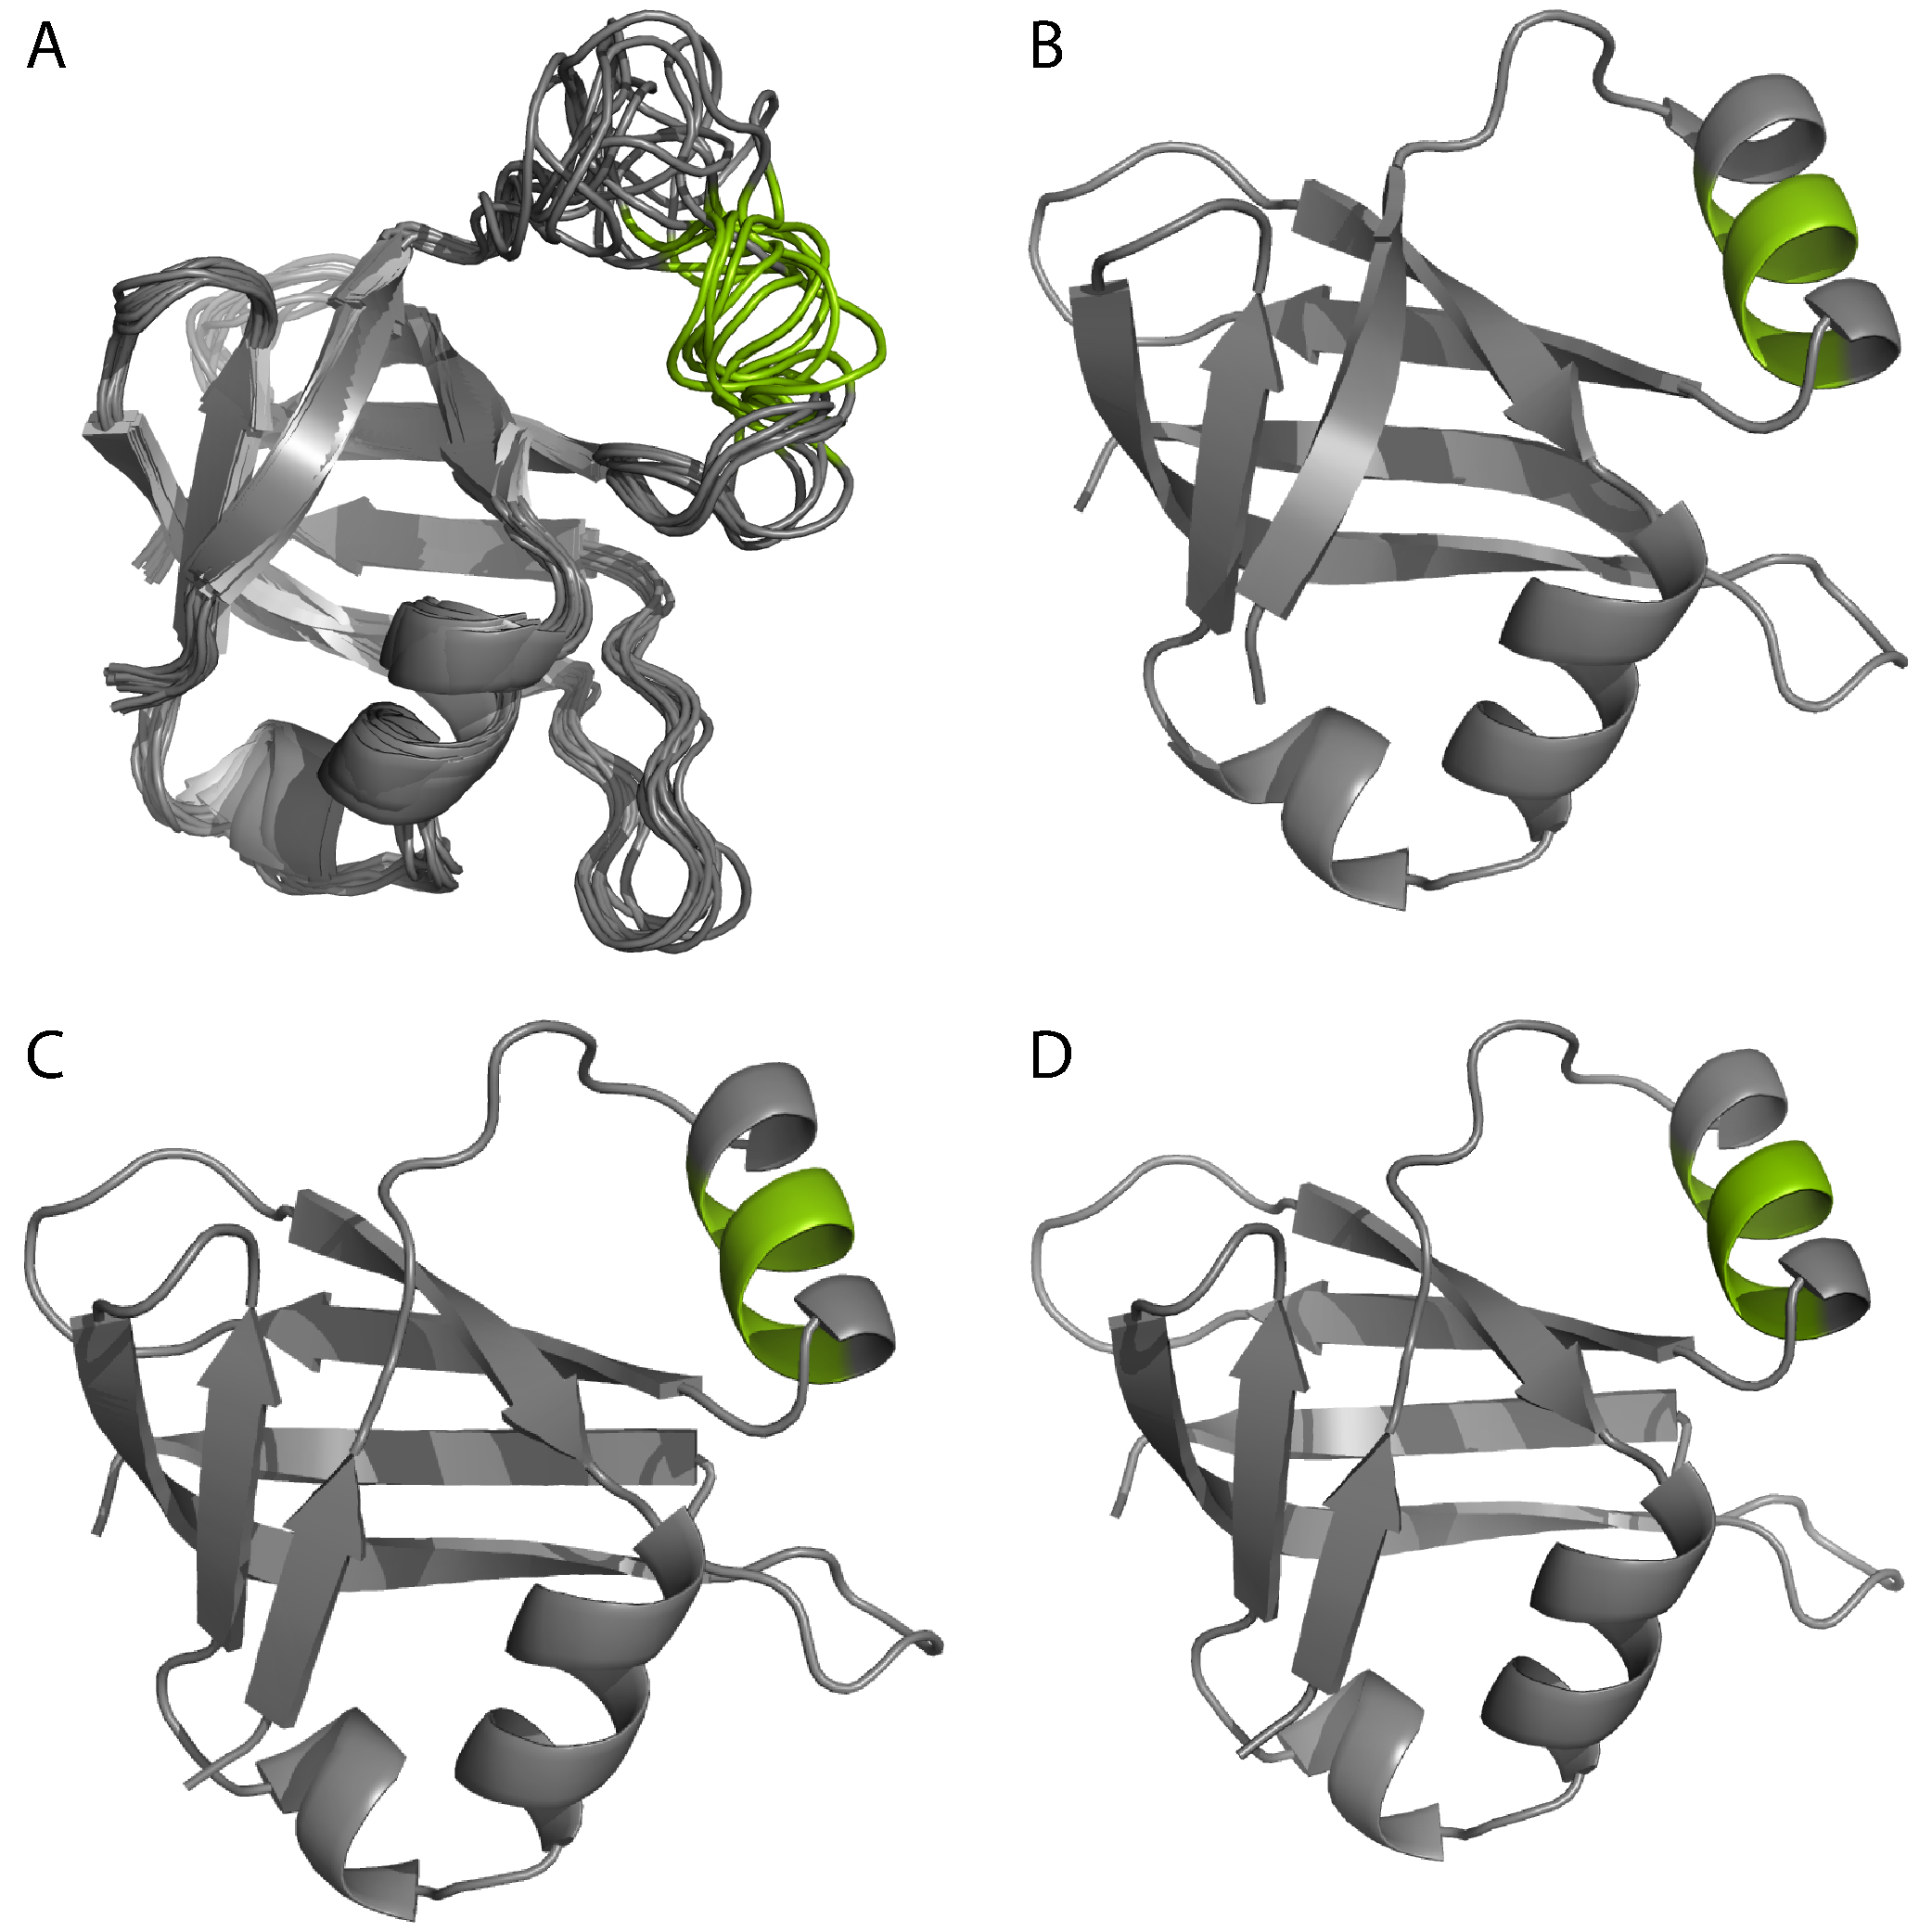
\includegraphics[width=0.85\linewidth]{figures/surrounding_notin_cryo.pdf}
    \caption{\textbf{Surrounding helix stabilisation into defined $\alpha$-helix by cryogenic temperatures in Cryo-EM in \textit{E. coli} ribosomal protein L25.} A) NMR ensemble (PDB id: 1B75 \cite{stoldt_nmr_1998}), with highlighted region indicating region with mixed ``Surrounding helix'' and ``Core helix'' for Constava's window sampling sizes 3 and 25, calculated on the corresponding MD simulation in \cite{gavalda-garcia_data-driven_2024} (dataframes in \burl{https://doi.org/10.5281/zenodo.10371447}) 
    B) Cryo-EM structure (PDB id: 8CGK \cite{paternoga_structural_2023}, chain W) with the same highlighted region adopting a canonical $\alpha$-helix conformation. 
    C) AlphaFold2 model of the protein (\burl{https://alphafold.ebi.ac.uk/entry/P68919}). The highlighted region is canonically folded, as in Cryo-EM. 
    D) AlphaFold3 model of the protein (calculated on \burl{https://alphafoldserver.com/} with sequence from UniProt id: P68919). The highlighted region is also canonically folded, as in Cryo-EM. 
    }
    \label{fig:discussion:surrhelix_vs_xray}
\end{figure}

The PDFs defining each conformational state are inversely related to their free energy landscape, where higher densities on a PDF denote thermodynamically favourable energy minima. If each conformational state is viewed as a local conformation macro-state, the state's likelihood maxima (or energy minima) in each PDF describe local conformation micro-states. ``Core'' conformational states, especially the ``Core helix'', exhibit very few micro-states within the macro-state, whereas ``Surrounding'' conformational states show a greater number of micro-states. Conformational states with more micro-states and thus broader probability densities (\textit{e.g.} ``Surrounding helix'') are more dynamic due to their flatter energy landscapes and lower energy barriers between minima (as illustrated by transitions in an energy landscape in \figref{fig:chapter1:landscape}). This facilitates transitions among multiple geometries in the backbone dihedral space. In contrast, conformational states with fewer micro-states indicate a more constrained energy landscape, with higher energy barriers between minima and, therefore, less dynamic behaviours. 

\textcolor{red}{The conformational states associated with the flattest energy landscapes in this work are labelled as ``Turn'' and ``Other''. Residues used to fit their probability density functions (PDFs) are flexible, as indicated by their chemical shifts, and are assigned either ``Turn'' or ``Other'' according to consensus STRIDE secondary structure assignments (detailed criteria in \tableref{tab:parameters_explanation}). Notably, the ``Other'' assignment corresponds to a consensus STRIDE coil assignment. We selected the term ``Other'' intentionally, to avoid restrictive definitions for these residues; STRIDE assigns the label coil when a residue does not fit any other structural category. Thus, to better represent the nature of highly dynamic residues without implying they are a mere fallback category, we opted for the nomenclature ``Other''.}


\subsection{Sampling of Likelihood Vectors to Calculate Propensities}

For a single pair of backbone dihedrals, the trained PDFs infer a six-dimensional vector that describes the likelihood of the amino acid existing in each conformational state, rather than assigning a single label, as traditional secondary structure methods do. Since the PDFs for all six conformational states extend and overlap along the entirety of the backbone dihedral space, a coordinate will generally present non-zero likelihoods for multiple conformational states (\figref{fig:kernels_energy}). By sampling multiple vectors, the Constava method is able to assign amino acid conformational state propensities. At smaller sampling sizes, it can describe an amino acid's propensities to exist in each conformational state. At larger sample sizes, it can describe more unique, preferred conformational states that amino acids like to adopt. For time-series protein structural ensembles (\textit{e.g.} generated with Molecular Dynamics (MD) simulations), sliding window sampling is preferred, as it can also highlight transition events between conformational states. Constava can also display the propensities for each sampling window, offering a more detailed analysis of conformational transition events. 

With Constava, local conformations can now be defined in a continuous vector space rather than in a class. This vector's dimensions are the \gls{dynamics}-informed, previously discussed conformational states.
Such definition expands and refines the dynamic definition of local conformation further, not only re-defining conformational states from ensembles in physiological temperature, but also enabling the description of local conformation as a vector of all their propensities. 


\subsection{Statistical Descriptions of Protein Conformation Represent Protein Populations Rather than Single Molecules.}

The statistical description of local conformations presents its own set of challenges, not found in secondary structure class assignment. Firstly, it is more conceptually convoluted to understand local conformation in a multi-dimensional spectrum than as a label, which can be a strong deterrent for the popular adoption of this method. Additionally, if the structural ensembles are obtained with NMR spectroscopy, the derived metrics describe the conformational states in which the residues of a population of proteins can exist, rather than those of a single molecule. 
If the structures are obtained from an MD simulation on a single molecule, they are dependent on the quality of the simulation's conformational sampling and can potentially be biased if the sampling is not representative of the protein's conformational diversity.


Finally, the definition of conformational states is subject to the criteria defined to select the data employed to fit their PDFs and their fitting parameters (\textit{e.g.} bandwidth). If these considerations are in discordance with the requirements of an analysis (\textit{e.g.} it is a single structure analysis), it might be preferred to classify local conformation in labels over applying a statistical description. 


\subsection{Conformational State Variability Reflects Diversity in the Conformational State Propensities Vectors}

When all vectors, from all samples, across every structure in a protein structural ensemble are considered, a metric of conformational state variability can be derived. This metric indicates, for an amino acid, how much its conformational state propensities vector varies across the samples. It is calculated as the root mean squared difference of every vector against the average vector across all samples (Equation \ref{eq_conf_state_var}). This conformational state variability metric describes a change in local conformation that describes a change in amino acid behaviour rather than a change in their backbone dihedrals or Cartesian coordinates. Additionally, all the functionalities here described can be applied to user-defined conformational states, for which we also provide support in Constava. This flexibility opens our method to be employed in use cases for which different conformational states are required, calculating conformational state propensities and variability from the custom, user-defined PDFs.

Though this metric can be employed on any protein ensemble, its application to time-series data obtained from MD simulations has produced more meaningful insights than on unsorted ensembles. This advantage arises from the sampling method, as time-series data can be sampled with a sliding window, which allows for the sampling of temporally adjacent structures, resulting in better-defined propensities. \textcolor{red}{Sliding window sampling allows the identification of conformational state transition events, propensities and variability under any environment in which the MD simulation is performed. Such transition events cannot be observed in metrics of protein flexibility, such as RMSF, CV or $S^{2}_{RCI}$, as they provide a measure across all models in an ensemble or frames in an MD simulation.} 

In contrast, when bootstrap sampling is used, non-adjacent likelihood vectors are grouped together, which can represent distinct behaviours, particularly for residues undergoing large conformational changes. Consequently, the sample method and size directly influence the values of conformational state variability, as the vectors used in its calculation are shaped by the chosen sampling strategy. We propose using sliding window sampling whenever possible, with sample sizes of 3 and 25 to represent the potential for existing in different conformational states and the preferred conformational state, respectively.

The dataset used to validate Constava, and to recommend sampling strategies, was generated using uniform MD simulation parameters. However, variations in experimental or computational setups might necessitate adjustments to these strategies to ensure accurate conformation descriptions. Since the predefined PDFs in Constava are based on NMR experimental data, an effective approach to select sampling strategies could involve benchmarking them against proteins with available NMR chemical shift data. Although this approach is not yet tested, we propose using ShiftCrypt \cite{orlando_shiftcrypt_2020} to determine a protein's conformational preferences. To apply this method, it is essential that some proteins in the dataset being analysed also have NMR chemical shift data. This allows ShiftCrypt to be used, and the resulting conformational state propensities can then be compared with those from our protein structural ensembles, helping to identify the most suitable sampling method for a given dataset.

% \textcolor{red}{A promising application of Constava is the exploration of transient conformations on IDPs and IDRs from MD simulations, similarly as shown in \figref{fig:md_timeseries}-c. When the overall propensities are calculated for each amino acid, across all samples, each residue can be represented by a 7-dimensional vector of conformational state propensities and variability. These profiles could be employed to assess adaptations in behaviour in evolutionarily-related proteins. A model built from related profiles may be used as a figurative ``barcode'' to search for further related regions, enabling a sequence-independent query scan of related IDPs and IDRs.}

\textcolor{red}{A promising application of Constava is exploring transient conformations of IDPs and IDRs from MD simulations, as illustrated in \figref{fig:md_timeseries}-c. By calculating the overall propensities for each amino acid across all samples, each residue can be represented by a 7-dimensional vector capturing conformational state propensities and variability. These profiles could be used to assess adaptive behaviours in evolutionarily related proteins. Additionally, a model built from related profiles could serve as a figurative ``barcode'' to identify further related regions, enabling a sequence-independent scan of similar IDPs and IDRs. This approach resembles searching for structural domains in ordered proteins, allowing for the identification of functional or structural analogues in the absence of a defined structure.}

% \textcolor{red}{Constava’s protein representation can detect NMR-defined conformational state propensities, including transition events using sliding window sampling, and assesses how readily a residue can adopt multiple conformational states. While ensemble averaging can be employed to calculate the average protein behaviour and infer dynamics from a protein ensemble, Constava provides a general, behaviour-based measurement of conformation and variability. This approach uniquely allows Constava to capture dynamic flexibility and highlight transition events within temporally resolved samples (\textit{e.g.} MD trajectories)—a capability not available in static or ensemble-average-based methods that lack temporal resolution.}

\textcolor{red}{Constava’s protein representation can detect NMR-defined conformational state propensities, including transition events using sliding window sampling, and assesses how readily a residue can adopt multiple conformational states. While ensemble averaging calculates average protein behaviour and infers dynamics from a set of static conformations, Constava provides a more generalised, behaviour-based measure of conformation and variability. This probabilistic approach uniquely allows Constava to capture dynamic flexibility and highlight transition events in temporally resolved samples (e.g., MD trajectories)—a capability unavailable in static or ensemble-average-based methods that lack temporal resolution and are constrained to population-level snapshots.}

% In contrast to ensemble averaging, which yields a single, averaged structure with variability inferred from atomic spread, Constava provides a behaviour-based measure of conformation and variability. This approach uniquely allows Constava to capture dynamic flexibility and highlight transition events within temporally resolved samples (\textit{e.g.} MD trajectories)—a capability not available in static or ensemble-average-based methods that lack temporal resolution.}

Finally, conformational state variability does not take into account which conformational states are involved in the conformational diversity, nor their conceptual similarity or lack thereof. This results in the equal treatment of vectors with swapping propensities between closely related conformational states (\textit{e.g.} ``Core helix'' and ``Surrounding helix'') and vectors with swapping propensities between more distant states (\textit{e.g.} ``Core helix'' and ``Core sheet''). Consequently, conformational state variability requires a parallel observation of conformational state propensities to identify which conformational states are driving the variability values.




\subsection{Constava's Availability and Immediate Perspectives}

Conformational state propensities and variability are introduced to the scientific community as new metrics for describing protein conformation at physiological temperatures. These metrics can be calculated using our method, Constava, which is available as a highly customisable Python package across multiple distribution channels and as a Galaxy Europe tool. We are currently exploring its integration into software tools aimed at studying protein structural ensembles.


\section{Evolution of b2BTools Deployment}

The comprehensive software deployment for Constava was made possible by applying lessons learned from the deployment of other tools developed in our research group, collectively known as the bio2Byte Tools (or b2BTools) suite. The development and deployment of these tools are discussed in detail in Chapter \ref{chapter:b2btools_deployment}, which encompasses the work presented in three articles addressing different stages of their deployment \cite{kagami_online_2021, kagami_b2btools_2021, gavalda-garcia_bio2byte_2024}. 


\subsection{The Initial Development of Each Tool}

Our research group has developed multiple predictors for protein biophysical properties as part of various research projects. These tools were created using contemporary versions of programming languages and dependencies, and their code was made publicly available along with an environment description to facilitate execution. This approach complies with the publishing guidelines of most scientific journals, providing, \textit{a priori}, sufficient information for software execution. However, in practice, installing software from the source code and dependency list can be challenging. It often necessitates creating a dedicated environment for each tool, as the dependencies may not be compatible with a user’s machine, requiring them to find alternative versions of these dependencies. In some cases, no suitable alternatives are available, rendering the software unusable. We believe these tools should be more easily and robustly accessible to the scientific community for two main reasons: 1) they were developed with public funding and should, therefore, be accessible to the public, and 2) their potential for rapid biophysical screening makes them valuable for prioritising resources and identifying potential targets during health emergencies.

\subsection{Publishing Results for Specific Problems}

During the height of the COVID-19 pandemic, we utilised our tools to analyse and publish data on all viral proteins and their homologs. Additionally, we implemented a method to describe biophysically allowed spaces based on Multiple Sequence Alignments (MSA) and the range of predicted values for each position. This approach can be employed to identify potential targets with narrow biophysically allowed spaces, which are theoretically more susceptible to disruption. By providing this critical information in a timely manner, we contributed to the global effort to mitigate the pandemic \cite{kagami_online_2021}. This method also bypassed issues related to software dependencies or programmatic literacy, as no execution was required by the end users.

More recently, we extended this approach by providing a comprehensive set of biophysical properties for the entire human proteome \cite{bio2byte_bio2bytes_nodate}, including an additional interpretation of protein disorder based on \cite{roca-martinez_challenges_2022}. We also applied this strategy from a user perspective, as described in \cite{gavalda-garcia_gradations_2024}, to reduce the computational expense of running AlphaFold2 on our largest dataset. However, this approach is limited to providing information on selected proteins.


\subsection{Creating a Web Server}

By building a web server, tools can be executed without the need for installation, leaving the execution-related nuances to the service providers. This approach had already been explored in our group with the single-tool execution of the DynaMine web server \cite{cilia_protein_2013, cilia_dynamine_2014}, developed prior to this thesis. During the preparation of the COVID-19 results \cite{kagami_online_2021}, we initiated the unification of our most popular tools to enable their joint execution on a new web server \cite{kagami_b2btools_2021}. This resulted in a service where users can submit their protein sequences and receive estimated protein biophysical metrics, along with interactive plots to facilitate interpretation. Additional features, such as execution on MSA files and a token-based programmatic interface, complemented the core service. However, web server execution carries inherent limitations. Firstly, as the web server's resources are limited, usage caps are often imposed to ensure fair access for all users \cite{abramson_accurate_2024, kagami_b2btools_2021}. Secondly, access to the tools is dependent on the continued availability of the online resource. These factors motivated us to explore deployment methods that ensure scalability and archival quality, thereby guaranteeing that our software remains accessible and is not limited in throughput.

\subsection{Distribution as a Python Package}

This marked the beginning of efforts to unify the bio2Byte tools into a single Python package, comprising the same tools included in the web server (Chapter \ref{chapter:b2btools_deployment}) \cite{gavalda-garcia_bio2byte_2024}. The primary challenge in this task was the unification of dependencies across different Python versions. This does not mean that every Python version must use the same dependency versions, which is highly unlikely to be feasible. Instead, it requires defining version ranges for dependencies specific to each Python version and ensuring that all code is written with syntax compatible across these versions. This process is significantly easier when the dependencies of these tools are minimal and consist of well-maintained packages (\textit{e.g.}, established tools like PyTorch \cite{paszke_pytorch_2019} or SciPy \cite{mckinney-proc-scipy-2010}), as packages with limited maintenance often impose more restrictive dependencies, complicating the deployment. We encountered such challenges during this process, which currently limits the incorporation of additional tools until more resources can be allocated for re-implementation without these restrictive dependencies.

Once the code is compatible across all Python versions and the dependencies are defined, an installable Python package can be created. With a well-configured Git repository, testing the package's build and execution can be automated. However, this usually incurs additional costs due to the computational resources used by the Git service during testing, so some prior local testing is recommended before the Git build. The package can then be uploaded to various distribution channels, such as PyPI \cite{pypi} or Bioconda \cite{gruning_bioconda_2018}, for local installation and execution on any supported machine. This approach simplifies software installation and updates but remains subject to the passage of time and the ongoing maintenance of dependencies.


\subsection{Archiving in Docker Images}

To ensure that our tools can be executed well into the future, they can be archived in Docker images \cite{merkel2014docker}. The deployment on Bioconda automatically creates a Docker image, which is then archived in Biocontainers \cite{da_veiga_leprevost_biocontainers_2017}, removing the need for independent Docker image creation. We implemented both approaches, making our tools available for all supported Python versions on Dockerhub (\burl{https://hub.docker.com/r/bio2byte/b2btools}) and for the latest Python version on Biocontainers (\burl{https://quay.io/repository/biocontainers/b2btools}). Each Docker image includes all the necessary requirements for the tools' execution, thereby ensuring their indefinite usability.


\subsection{Inclusion in Pipeline Creation Platforms}

The compartmentalisation of our software into a Docker image allows for its incorporation into pipelines as an independent, self-contained module. A well-known platform for pipeline creation is NextFlow \cite{di_tommaso_nextflow_2017}, with which we have successfully tested b2BTools as part of pipelines using our Docker images. This means the software is ready to be integrated into any pipeline, provided the user has sufficient knowledge to create the pipeline. To further facilitate its use in pipelines, we developed a Galaxy Europe \cite{afgan_galaxy_2018} tool based on a Biocontainers Docker image. Our tools can now be executed as part of pipelines without the need for programmatic literacy, either on the Galaxy Europe server or with Galaxy's local software. The current deployment of b2BTools ensures its usability across all levels of computational literacy, making it insensitive to software version changes and scalable.


\subsection{Challenges for Small Research Groups}

Improving the deployment status of a tool suite is particularly challenging for small research groups due to their limited resources. The creation of a web server, for instance, requires expertise that is often unrelated to the primary research focus of the group. This may necessitate hiring additional personnel for support tasks or outsourcing these tasks, which can strain the group's resources. Additionally, hosting and computation time are required to keep the services running, although some host institutions may offer their resources for these tasks. The additional funding needed to maintain a web server also poses a risk to its continuity, making it crucial for small groups to archive Docker images of their tools and integrate them into online pipeline platforms.

Another significant challenge for software developed by small research groups is the risk of not updating their tools to remain compatible with new software versions. Limited resources can deter other developers from using these tools as dependencies, given the uncertainty about their long-term support, especially when compared to well-established software. This presents a conundrum: while we advocate for the use of well-established, regularly updated software, we also offer a tool suite that has yet to demonstrate its long-term continuity and compatibility with newer dependencies. Although we are committed to maintaining good deployment practices, the natural turnover of staff and the fluctuation of funding pose risks to this commitment.

Given the increasing number of scientific software tools, universities and research institutions should consider creating specialised departments dedicated to updating and maintaining software produced by their researchers, even after they have left or retired. This would alleviate the pressure on researchers to secure funding for software maintenance and ensure the tool's availability and relevance to the scientific community for as long as needed.


\subsection{Current State and Perspectives}

Currently, our tools can be executed in a variety of ways: locally or in the cloud, programmatically or via a user interface, as an installed package, container, or pipeline. They are archived to ensure their long-term usability, their code is available, and they are well-documented. We are confident that the current versions are future-proof and will remain executable, at the very least as containers built from their Docker images.

We continue to improve and expand our tool suite. For example, we have recently added the interpretation of NMR chemical shifts with ShiftCrypt \cite{orlando_shiftcrypt_2020}, and we plan to further expand our catalogue. The predictors in our suite tackle different aspects of protein \gls{dynamics}, so including more of them in a single suite helps provide a holistic vision of protein \gls{dynamics}. These predictions have also proven to carry valuable information for diverse predictive tasks, as illustrated in Chapter \ref{chapter:ambiguous} \cite{roca-martinez_challenges_2022} and the interdependencies among tools in the suite itself (Supplementary Table 6.2). 
% (\suppfigref{tab:tool_dependencies}).

Additionally, we have introduced some MSA functionalities, which are available in the latest version, though some features are still under development. We anticipate the need to replace a specific dependency with more general code, which will facilitate updates to our tools and broaden their compatibility with various Python versions and packages. The web server is currently transitioning from employing a clone of our Git repository to utilising our Python package as its back-end. While these plans aim to enhance the functionality and robustness of our tools' deployment, the steps already taken ensure that their current capabilities will remain accessible to the scientific community over time.

\section{AlphaFold and Protein Dynamics}

The importance of scientific software has become increasingly evident in recent years, culminating in the development of AlphaFold and its subsequent versions. AlphaFold is a Machine Learning (ML) model for predicting protein structures from their sequences at resolutions comparable to experimentally determined structures. Its creation has revolutionised structural biology, representing a once-in-a-generation technological leap that has advanced the field by decades beyond its anticipated progression. Some have even described AlphaFold as the most significant application of Artificial Intelligence (\gls{artificialintelligence}) to date \cite{toews_alphafold_nodate}. The scientific repercussions of having hundreds of millions of high quality predicted protein structures have just begun, and are expected to revolutionise medicine and life sciences. The field of protein structure prediction has since caught up, and most modern protein structure predictors are now based on deep neural networks (DNNs). In other words, these tools feature neural networks (NNs) with multiple large-dimensional layers and complex architectures.


\subsection{Prediction of Protein Native Structures}

Such models require vast amounts of data for their training, typically sourced from public protein structure and sequence databases. These databases, populated through the contributions of thousands of scientists and curators, are fundamental to enabling this new wave of DNN-based predictors. AlphaFold was trained exclusively on X-ray crystallography and Cryo-EM structures, both of which provide single protein structures that represent their minimum energy native state. NMR-derived structures were excluded, thus limiting the training data to those obtained under dehydrated, cryogenic conditions. Earlier in this discussion, we highlighted how these conditions can influence a protein's conformation (\figref{fig:discussion:surrhelix_vs_xray} A \& B), potentially forcing dynamic conformations into more rigid ones. Consequently, AlphaFold predicts structures that closely resemble those derived from X-ray and Cryo-EM data (\figref{fig:discussion:surrhelix_vs_xray} C \& D). 

\textcolor{red}{Due to training predominantly on rigid structures, AlphaFold models often predict flexible regions as defined secondary structures. AlphaFold 3 introduced a diffusion-based architecture, which, while enhancing predictive flexibility, is more prone to generating artifacts, formally termed ``hallucinations'' in generative machine learning models. Their work addresses these ``hallucinations'', outlining strategies designed to minimise them \cite{abramson_accurate_2024}. In our analysis, we did not observe notable differences in ``hallucinations'' between AlphaFold 2 and AlphaFold 3; however, this was not a formal, exhaustive comparison. }

As single structures, both the training data and AlphaFold's predictions do not explicitly account for a protein's flexibility. However, its metric for predicted local distance difference test (pLDDT) has been shown to be influenced by protein flexibility \cite{saldano_impact_2022}. In Chapter \ref{chapter:plddt}, we explore the relationship between pLDDT, and experimental and computational metrics of protein \gls{dynamics} to further elucidate its significance and nuances.


\subsection{AlphaFold2's pLDDT Relation to Extremes in Protein Dynamics}

A residue's pLDDT measures the confidence with which AlphaFold has predicted the location of that residue. High pLDDT indicates high predictive confidence, while low pLDDT suggests lower confidence. Our work in Chapter \ref{chapter:plddt} \cite{gavalda-garcia_gradations_2024} suggests a correlation between pLDDT values and experimental metrics for protein \gls{dynamics}, specifically the $S^{2}_{\text{RCI}}$ and $S^{2}$ order parameters.

The $S^{2}$ order parameter is an experimental measure of order from NMR backbone relaxation experiments, typically reflecting the degree of order in amino acid motions on the pico- and nano-second timescale. High $S^{2}$ values indicate restricted amino acid motions, which are often associated with regular secondary structures and/or motion constraints imposed by the amino acid's local environment. Conversely, low $S^{2}$ values suggest more unrestricted motions, allowing the amino acid to explore a wider range of orientations. Due to the experimental challenges in directly obtaining $S^{2}$, an approximation, $S^{2}_{\text{RCI}}$, can be derived from the Random Coil Index (RCI). This metric interprets RCI data to provide a measure of backbone flexibility on a scale that resembles $S^{2}$, facilitating its interpretation.

In this context, flexibility is defined as the ability of a residue to adopt multiple conformations, typically assessed over longer timescales than those captured by $S^{2}$. Therefore, while $S^{2}_{\text{RCI}}$ measures the breadth of an amino acid's conformational landscape, the inverse of $S^{2}$ reflects the rate at which the amino acid transitions between different regions of this landscape.

Generally, high pLDDT corresponds to amino acids that do not change in coordinates, therefore indicating high order or rigidity. Low pLDDT usually corresponds to amino acids that do not occupy a fixed spatial location. We observed deviations from this trend, where the NMR-derived dynamic measurements of amino acids contrast with the expected pLDDT-assumed dynamism. We found experimentally determined flexible amino acids from interpreted RCI data \cite{orlando_shiftcrypt_2020} with corresponding high pLDDT values (\figref{fig:plddt_vs_shiftcrypt_undivided}). We then identified long contigs of such amino acids and mapped them to static experimental structures obtained by X-ray crystallography or Cryo-EM. We found an example, the mouse Cytohesin-3 or Grp1 (UniProt accession code O08967), where such a contig matched a region with no defined secondary structure, but seemed to be stabilised by the binding of a ligand (\figref{fig:shiftcrypt_and_allosterism}). Upon closer inspection of all static experimental structures available in the Protein Data Bank (PDB), we observed the presence of its ligand Ins(1,3,4,5)P\textsubscript{4}, or an analogous molecule, in all entries. All entries were also published before AlphaFold2's cut-off date for the creation of its training dataset, which indicates that they were all considered in the creation of AlphaFold2's training dataset. 

The processing of AlphaFold2's training data deletes any ligand from the structure, and in the case of Cytohesin-3, it leaves a long, unstructured protein region fixed in space as if the ligand was present. We hypothesise that the immobility of coordinates for this region was captured either in AlphaFold2's training process or template usage for prediction (\figref{fig:chapter1:af2_structure}), resulting in high predictive confidence and thereby high pLDDT values. In this case, the interpretation of pLDDT as a metric of rigidity would be misleading, as the predicted unbound form indicates rigidity characteristic of its bound form. Such behaviour in this specific entry is also present in AlphaFold3 (\figref{fig:discussion:af3_pocket}), which has the capacity to predict the location of some ligands and ions in its produced predicted protein structures \cite{abramson_accurate_2024}. Further exploration of these mismatching interpreted RCI and pLDDT metrics will be required to identify more artifacts derived from AlphaFold's data processing. 


\begin{figure}[tbh]
    \centering
    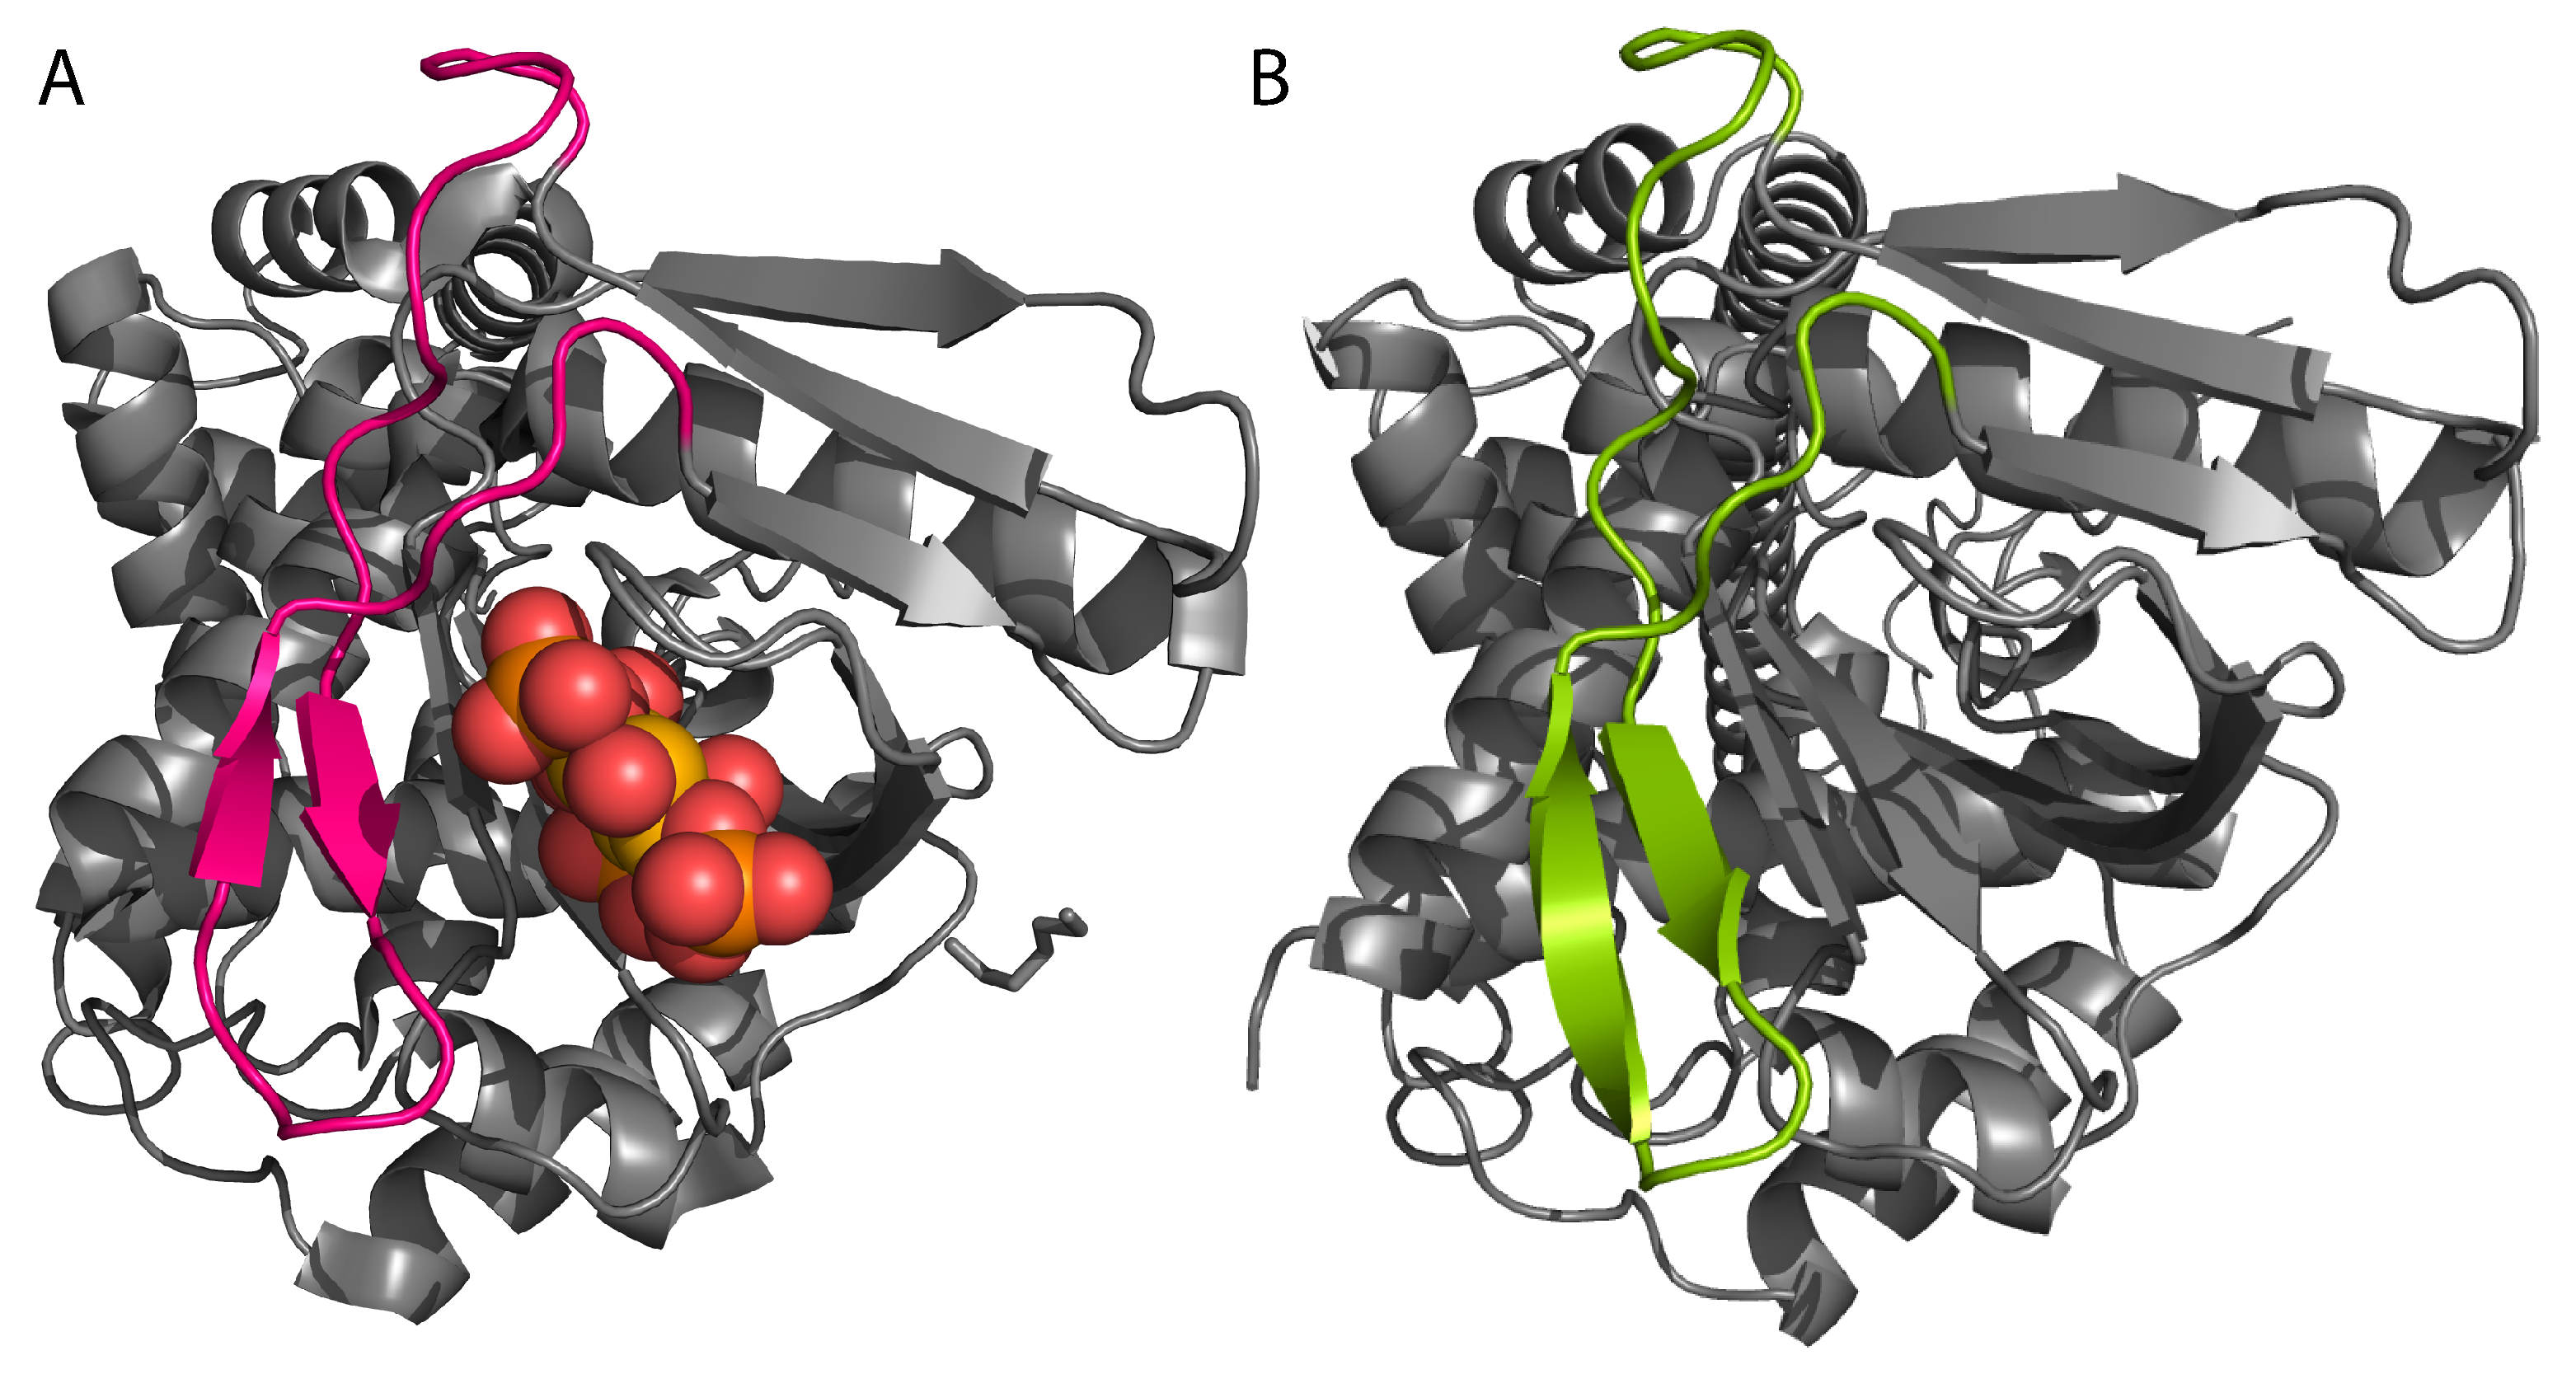
\includegraphics[width=1\linewidth]{figures/af3_pocket.pdf}
    \caption{\textbf{Mouse Cytohesin 3 binding pocket in experimental structure and AlphaFold3.} A) Experimental structure (PDB id: 2R0D \cite{dinitto_structural_2007}) with Ins(1,3,4,5)P\textsubscript{4} bound. Highlighted is the loop which features a long continuous segment of high pLDDT with ShiftCrypt values which show disorder. B) AlphaFold3 predicted structure. Highlighted is the same region as in A). The space occupied by Ins(1,3,4,5)P\textsubscript{4} in A) is present, in the absence of the ligand, in B).}
    \label{fig:discussion:af3_pocket}
\end{figure}


\subsection{pLDDT Does Not Accurately Reflect Gradations in Protein Dynamics}

We thereby find that pLDDT has a binary relationship with $S^{2}$ and $S^{2}_{\text{RCI}}$, where clearly rigid and clearly dynamic residues usually have high and low pLDDT values, respectively. Considering the largest dataset, with values for $S^{2}_{\text{RCI}}$, the overall correlation of pLDDT with $S^{2}_{\text{RCI}}$ is weak, especially when data is considered in strata (\tableref{table:pearson_metrics}). The stronger correlation for the full data spectrum than for strata indicates that pLDDT can better describe the extremes of protein \gls{dynamics}, but fails to describe fine gradations in \gls{dynamics}. Such results are coherent with the relation of pLDDT with predicted $S^{2}_{\text{RCI}}$, described in Chapter \ref{chapter:ambiguous} \cite{roca-martinez_challenges_2022}, where two high-density regions could be identified for predicted backbone \gls{dynamics} (\figref{fig:chapter5:fig5}). Constava's conformational state variability also shows similar trends, with only high pLDDT residues featuring low conformational state variability, but both mid and low pLDDT featuring predominantly high variability and low correlation along the whole range of values (\figref{fig:plddt_vs_conf_state_undivided}). This indicates a sharp change in behaviour from different pLDDT regions, rather than a gradation describing protein dynamic behaviour.

\subsection{Amino Acids with Multiple Conformations Tend to Feature Lower pLDDT}

In addition to pLDDT's relation to Constava's conformational state variability, we also observed that residues with the same secondary structure assignment across the entirety of the an NMR ensemble tend to have higher pLDDT values (Supplementary Fig. 5.10 A, D, G \& J). 
% (\suppfigref{fig:unique_and_or_cons} A, D, G \& J). 
Interestingly, this is also true for Coil and Turn, which are inherently unstructured, indicating that Coil and Turn residues that do not experience diversity in secondary structures are predicted more confidently by AlphaFold2 than those which do. Additionally, for every secondary structure type, those residues for which their predicted AlphaFold2 secondary structure matches the consensus secondary structure of the NMR ensemble also features higher pLDDT distributions than when these assignments mismatch (Supplementary Fig. 5.9 A, D \& G). 
% (\suppfigref{fig:af2_nmr_fold_missmatch} A, D \& G). 

Moreover, the match between AlphaFold2 and consensus NMR assignments results, for $\alpha$-Helix and $\beta$-Sheet, in higher pLDDT assignments than those with unique NMR assignments and mismatched AlphaFold2 assignments. The opposite is true for Coil and Turn residues, where a unique NMR assignment was more important than a matching AlphaFold2 assignment to obtain higher pLDDT distributions (Supplementary Fig. 5.11 A, D, G \& J).
% (\suppfigref{fig:unique_and_or_cons_match_af2} A, D, G \& J).
This is probably explained by the rigidisation of defined secondary structures into more stable forms under cryogenic conditions (\figref{fig:discussion:surrhelix_vs_xray}). AlphaFold replicates these rigid conformations and results in the assignment of the consensus NMR secondary structures, as it is the favourable one in cryogenic conditions. Overall, AlphaFold2 clearly shows a tendency for assigning higher pLDDT values to residues with unique secondary structure assignments across all structures in NMR structural ensembles.

Additionally, we have applied the Constava method to conformations generated with AlphaFlow \cite{jing_alphafold_2024}, a method that employs elements from AlphaFold's models to generate structural ensembles. Constava can be employed to compare structural ensembles and their conformational state propensities and variabilities, in this case between MD- and AlpaFlow-derived ensembles. From our limited testing, the ensembles generated with AlphaFlow seemed to overestimate protein conformational diversity compared to those obtained from MD simulations. This is reflected in more distributed conformational state propensities and therefore higher conformational state variability. Further, thorough testing is needed to assess more detailed differences between these ensembles and therefore the characteristics of AlphaFold-derived ensembles.


\section{Future Perspectives}

The work presented in this thesis opens the door to follow-up projects in several directions. The Constava software introduced new metrics to probabilistically describe protein conformation and its variability. This method is the product of several iterations, each with its own vision and strategies. During earlier stages, a branch of the project envisioned training a ML model to estimate Constava's metrics from amino acid sequence. Although these attempts were not immediately successful, they helped identify flaws in the definitions at each iteration. The final iteration of Constava focused on the description and thorough validation of the method, relegating the training of the estimator. While early attempts to create such an estimator have not yet achieved satisfactory performance, the project remains plausible. If these efforts succeed, we could see the expansion of bio2Byte Tools with a novel estimator of protein biophysics from amino acid sequences.

The expansion of bio2Byte Tools currently faces challenges arising from dependencies on crucial tools within the suite. These challenges have highlighted the necessity of generalising methods as much as possible and reducing external dependencies, particularly those lacking consistent updates to maintain compatibility with other contemporary software. A crucial and increasingly urgent task will be the re-implementation of multiple functions from obsolete dependencies into more generic code. Delaying this will likely result in the suite becoming another ``obsolete dependency'' itself. This is likely not a trivial process and will require the combined expertise of both technical and scientific staff.

Finally, the analysis of AlphaFold2's pLDDT leaves two immediate open paths for further research. First, a focused exploration of regions with conflicting NMR and AlphaFold \gls{dynamics} and conformations could provide deeper insights into the model's biases. We have shown general trends, supported by a key example illustrating the hypothetical effects of AlphaFold2's data processing pipeline, but further work could solidify and expand our interpretation. Secondly, some aspects of the study were limited by the daily job caps for generating AlphaFold3 predictions. It will be interesting to compare the current AlphaFold2 results with those of AlphaFold3 considering the recent publication of its code as open source \cite{callaway_ai_2024}. 
% when the method's code becomes public, the job cap is lifted, or a database with UniProt sequences is published, as was previously done for AlphaFold2.


\section{Closing Statement}

This thesis has introduced a new method to probabilistically describe protein conformation and its diversity, outlined a path for transforming outdated scientific tools into FAIR software, and explored the relationship between AlphaFold2 (and AlphaFold3, when possible) with protein \gls{dynamics} and conformation. The conclusions reached here open up new research avenues, some of which have been described above. These are aligned with the expertise and research lines of the bio2Byte group and will surely be further explored.

